\documentclass{article}

\usepackage{amsmath,amssymb}
\usepackage{tikz}
\usetikzlibrary{er,positioning}
\usepackage{pgfplots}
\usepackage{xcolor}
\usepackage[left=2.1cm,right=3.1cm,bottom=3cm,footskip=0.75cm,headsep=0.5cm]{geometry}
\usepackage{enumerate}
\usepackage{enumitem}
\usepackage{marvosym}
\usepackage{tabularx}
\usepackage{parskip}
\usepackage{longtable}

\usepackage{listings}
\definecolor{lightlightgray}{rgb}{0.95,0.95,0.95}
\definecolor{lila}{rgb}{0.8,0,0.8}
\definecolor{mygray}{rgb}{0.5,0.5,0.5}
\definecolor{mygreen}{rgb}{0,0.8,0.26}
\lstdefinestyle{sql} {language=sql}
\lstdefinestyle{python} {language=python, morekeywords={with, as}}
\lstset{basicstyle=\ttfamily,
	keywordstyle=\color{lila},
	commentstyle=\color{lightgray},
	stringstyle=\color{mygreen}\ttfamily,
	backgroundcolor=\color{white},
	showstringspaces=false,
	numbers=left,
	numbersep=10pt,
	numberstyle=\color{mygray}\ttfamily,
	identifierstyle=\color{blue},
	xleftmargin=.1\textwidth, 
	%xrightmargin=.1\textwidth,
	escapechar=§,
	breaklines=true,
	postbreak=\mbox{\space}
}

\usepackage[utf8]{inputenc}

\renewcommand*{\arraystretch}{1.4}

\newcolumntype{L}[1]{>{\raggedright\arraybackslash}p{#1}}
\newcolumntype{R}[1]{>{\raggedleft\arraybackslash}p{#1}}
\newcolumntype{C}[1]{>{\centering\let\newline\\\arraybackslash\hspace{0pt}}m{#1}}

\newcommand{\E}{\mathbb{E}}
\DeclareMathOperator{\rk}{rk}
\DeclareMathOperator{\Var}{Var}
\DeclareMathOperator{\Cov}{Cov}

\def\ojoin{\setbox0=\hbox{$\bowtie$}%
	\rule[-.02ex]{.25em}{.4pt}\llap{\rule[\ht0]{.25em}{.4pt}}}
\def\leftouterjoin{\mathbin{\ojoin\mkern-5.8mu\bowtie}}
\def\rightouterjoin{\mathbin{\bowtie\mkern-5.8mu\ojoin}}
\def\fullouterjoin{\mathbin{\ojoin\mkern-5.8mu\bowtie\mkern-5.8mu\ojoin}}

\title{\textbf{Datenbanken, Hands-on 3}}
\author{\textsc{Henry Haustein}}
\date{}

\begin{document}
	\maketitle

	\section*{Aufgabe 1}
	Ich habe ein Python-Skript geschrieben, was die Aufgaben löst. Dafür habe ich die Bibliothek \texttt{networkx} für die Graphen-Implementation und \texttt{matplotlib} zum Zeichnen des Graphen benutzt.
	\begin{lstlisting}[style=python, tabsize=2]
import networkx as nx
import matplotlib.pyplot as plt

filename = "graph_17.txt"

def reachableNodes(graph, start, exploredNodes):
	for vertex in graph.neighbors(start):
		if vertex not in exploredNodes:
			exploredNodes.append(vertex)
			moreVertices = reachableNodes(graph, vertex, exploredNodes)
			exploredNodes.extend(moreVertices)
	# gleich Duplikate herausfiltern um Rechenleistung und RAM zu sparen
	return list(set(exploredNodes))

def getNodesPartOfCycle(graph):
	nodesPartOfCycle = []
	for vertex in G.nodes:
		if vertex not in nodesPartOfCycle:
			if vertex in reachableNodes(graph, vertex, []):
				nodesPartOfCycle.append(vertex)
	return nodesPartOfCycle

# Zuordnung zwischen einem Knoten und dem Zeitstempel
verticesWithTimestamp = {}

print("Start Einlesen der Kanten")
with open(filename) as f:
	lines = f.read().splitlines()
	for line in lines:
		if line == "<<objects>>":
			# Start der Liste an Knoten
			numberVertices = 0
			continue
		if line == "<<edges>>":
			# Ende der Liste an Knoten
			break
		numberVertices = numberVertices + 1
		id = line.split("\t")[0]
		timestamp = line.split("\t")[1]
		verticesWithTimestamp.update({id: timestamp})


G = nx.DiGraph()
print("Start Hinzufuegen der Knoten zum Graphen")
G.add_nodes_from(list(verticesWithTimestamp.keys()))

print("Start Hinzufuegen der Kanten zum Graphen")
# Datei wird zeilenweise eingelesen, aber der fuer uns wichtige Inhalt kommt erst, wenn "<<edges>>" einmal aufgetaucht ist
processEdges = False
with open(filename) as f:
	lines = f.read().splitlines()
	for line in lines:
		if processEdges:
			try:
				start = line.split("\t")[0]
				enden = line.split("\t")[1].split(",")
				for ende in enden:
					G.add_edge(start, ende)
			except Exception as e:
				# falls ein Knoten mal keine Enden hat, wird die Zeile nicht bearbeitet - ist ja auch nicht notwendig
				pass
		if line == "<<edges>>":
			processEdges = True


# Zeichnen des Graphen
plt.box(False)
nx.draw_networkx(G)
plt.show()

removedNodes = []

while True:
	nodesPartOfCycle = getNodesPartOfCycle(G)
	NodesWithTimestamps = {}
	if len(nodesPartOfCycle) > 0:
		print("========================= Zyklus gefunden =========================")
		# es gibt Zyklen
		print("Aktuelle Knoten, die Teil eines Zyklus sind: " + str(nodesPartOfCycle))
		for elem in nodesPartOfCycle:
			# Zu jedem Knoten in einem Zyklus suchen wir uns den passenden Timestamp
			NodesWithTimestamps.update({elem: verticesWithTimestamp[elem]})
		# Sortieren nach aufsteigendem Timestamp
		NodesWithTimestamps = dict(sorted(NodesWithTimestamps.items(), key=lambda item: item[1]))
		print("Sortierte Liste an Knoten mit ihrem Zeitstempel: " + str(NodesWithTimestamps))
		# letztes Element ist der juengste Knoten
		youngestNode = list(NodesWithTimestamps)[-1]
		print("Juengster Knoten: " + str(youngestNode))
		removedNodes.append(youngestNode)
		G.remove_node(youngestNode)
	else:
		# es gibt keine Zyklen mehr -> Programm ist fertig
		print("========================= Programm fertig =========================")
		print("Sortierte Liste an entfernten Knoten: " + str(sorted([int(node) for node in removedNodes])))
		plt.box(False)
		nx.draw_networkx(G)
		plt.show()
		break
	\end{lstlisting}
	
	In Zeile 4 muss der Dateiname der Datei mit der Repräsentation des Graphen eingetragen werden. Unsere Gruppe hatten den Graphen 17 zu bearbeiten, der Graph sieht vor der Bearbeitung so aus:
	\begin{center}
		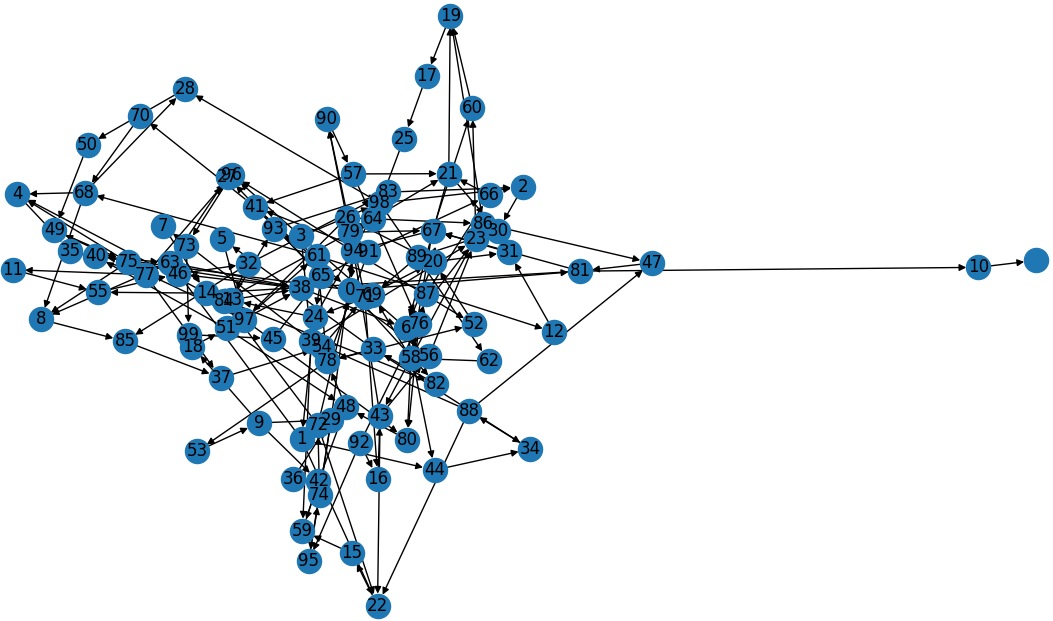
\includegraphics[width=0.75\textwidth]{./vorher}
	\end{center}
	Und so nach dem Algorithmus:
	\begin{center}
		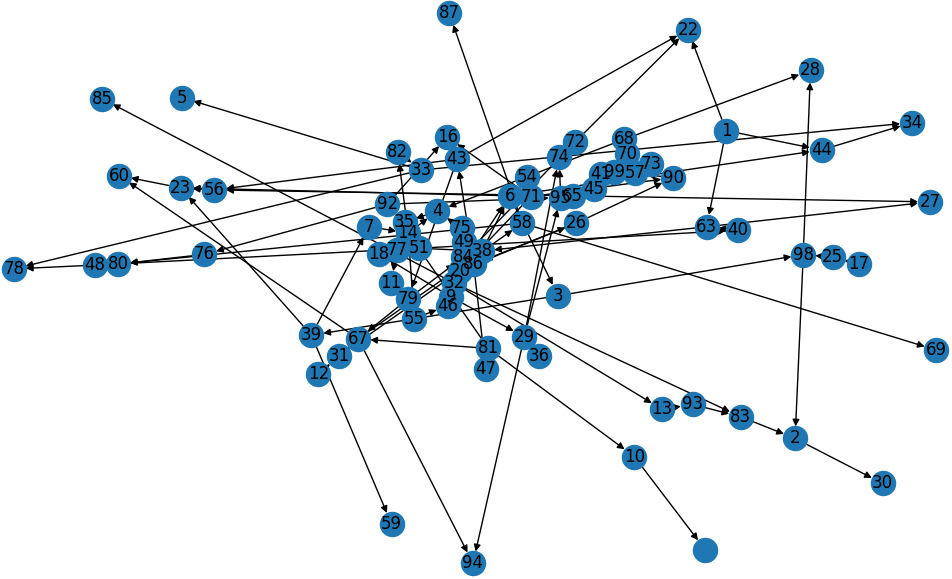
\includegraphics[width=0.75\textwidth]{./nachher}
	\end{center}
	Insgesamt wurden die folgenden Knoten entfernt (hier als Listenrepräsentation): \texttt{[0, 8, 15, 19, 21, 24, 37, 42, 50, 52, 53, 61, 62, 64, 66, 88, 89, 91, 96, 97]}
	
\end{document}